% question 7
\qs{}{
    How many students does International School of the National Artistic Arts University have?
}

Query the student table with a \texttt{WHERE} clause that only asks for students that have the ISNAA University in their records. 
\vspace{\baselineskip}

\sol{}
\noindent\line(1, 0){0.89\linewidth}
\begin{verbatim}
select count(*) as Students from student where stud_hs_name =
"International School of the National Artistic Arts University";
\end{verbatim}
\noindent\line(1, 0){\linewidth}

\begin{figure}[H]
    \centering
    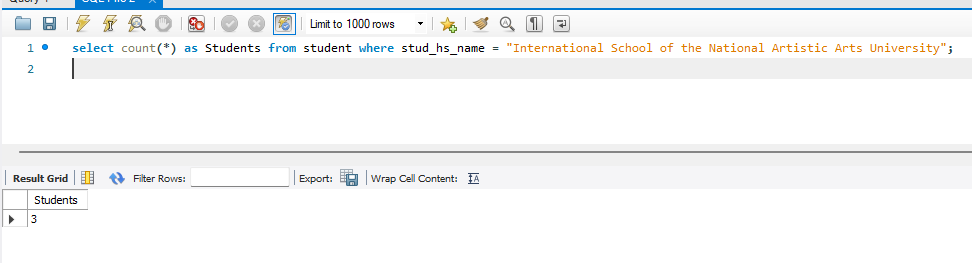
\includegraphics[width=0.7\linewidth]{images/q7.png}
    \caption{Question 7 Query and Output}
\end{figure}
